\definecolor{tttttt}{rgb}{0.2,0.2,0.2}
\definecolor{ttttff}{rgb}{0.2,0.2,1}

%dash pattern=on 5pt off 2pt
%[fill = white, rounded corners = 5pt, inner sep=0.8pt]
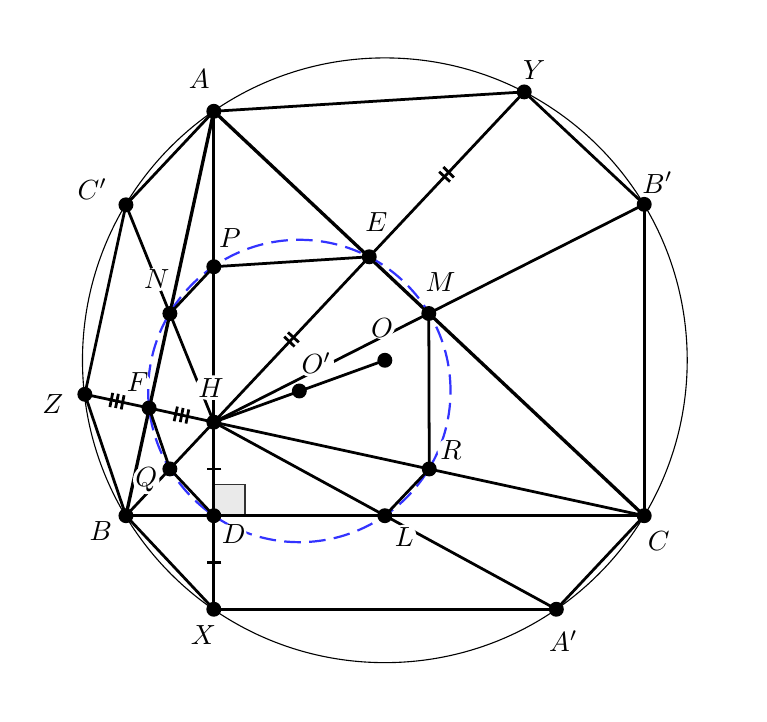
\begin{tikzpicture}[scale = 0.60]
    \clip(-3.71,-5.49) rectangle (11.35,8.61);
    \draw[color=tttttt,fill=tttttt,fill opacity=0.1] (0.89,-1.72) -- (0.89,-1.06) -- (0.23,-1.06) -- (0.23,-1.72) -- cycle;
    \draw [line width=1.2pt] (-1.63,-1.72)-- (9.34,-1.72);
    \draw [line width=1.2pt] (0.23,6.84)-- (9.34,-1.72);
    \draw [line width=1.2pt] (0.23,6.84)-- (-1.63,-1.72);
    \draw(3.85,1.57) circle (6.4cm);
    \draw [line width=0.8pt, dash pattern=on 6pt off 3pt, color=ttttff] (2.04,0.92) circle (3.2cm);
    \draw [line width=1pt] (0.23,0.26)-- (7.48,-3.7);
    \draw [line width=1pt] (0.23,0.26)-- (9.34,4.87);
    \draw [line width=1pt] (0.23,0.26)-- (-1.63,4.86);
    \draw [line width=1pt] (0.23,-3.7)-- (7.48,-3.7);
    \draw [line width=1pt] (7.48,-3.7)-- (9.34,-1.72);
    \draw [line width=1pt] (9.34,-1.72)-- (9.34,4.87);
    \draw [line width=1pt] (9.34,4.87)-- (6.8,7.25);
    \draw [line width=1pt] (6.8,7.25)-- (0.23,6.84);
    \draw [line width=1pt] (0.23,6.84)-- (-1.63,4.86);
    \draw [line width=1pt] (-1.63,4.86)-- (-2.5,0.85);
    \draw [line width=1pt] (-2.5,0.85)-- (-1.63,-1.72);
    \draw [line width=1pt] (0.23,0.26)-- (3.85,1.57);
    \draw [line width=1pt] (0.23,6.84)-- (0.23,0.26);
    \draw [line width=1pt] (-1.63,-1.72)-- (0.23,0.26);
    \draw [line width=1pt] (0.23,0.26)-- (9.34,-1.72);
    \draw [line width=1pt] (0.23,0.26)-- (0.23,-1.72);
    \draw [line width=1pt] (0.39,-0.73) -- (0.08,-0.73);
    \draw [line width=1pt] (0.23,-1.72)-- (0.23,-3.7);
    \draw [line width=1pt] (0.39,-2.71) -- (0.08,-2.71);
    \draw [line width=1pt] (-2.5,0.85)-- (-1.14,0.56);
    \draw [line width=1pt] (-1.91,0.88) -- (-1.97,0.58);
    \draw [line width=1pt] (-1.79,0.86) -- (-1.85,0.56);
    \draw [line width=1pt] (-1.67,0.83) -- (-1.73,0.53);
    \draw [line width=1pt] (-1.14,0.56)-- (0.23,0.26);
    \draw [line width=1pt] (-0.54,0.59) -- (-0.61,0.28);
    \draw [line width=1pt] (-0.42,0.56) -- (-0.48,0.26);
    \draw [line width=1pt] (-0.3,0.53) -- (-0.36,0.23);
    \draw [line width=1pt] (0.23,0.26)-- (3.52,3.76);
    \draw [line width=1pt] (1.72,2.07) -- (1.94,1.86);
    \draw [line width=1pt] (1.8,2.16) -- (2.03,1.95);
    \draw [line width=1pt] (3.52,3.76)-- (6.8,7.25);
    \draw [line width=1pt] (5,5.56) -- (5.23,5.35);
    \draw [line width=1pt] (5.09,5.66) -- (5.31,5.44);
    \draw [line width=1pt] (3.52,3.76)-- (0.23,3.55);
    \draw [line width=1pt] (0.23,3.55)-- (-0.7,2.56);
    \draw [line width=1pt] (-1.14,0.56)-- (-0.7,-0.73);
    \draw [line width=1pt] (-0.7,-0.73)-- (0.23,-1.72);
    \draw [line width=1pt] (3.85,-1.72)-- (4.79,-0.73);
    \draw [line width=1pt] (4.79,-0.73)-- (4.78,2.56);
    \draw [line width=1pt] (-1.63,-1.72)-- (0.23,-3.7);
    \begin{scriptsize}
        \normalsize
        \fill [color=black] (0.23,6.84) circle (4.5pt);
        \draw[color=black] (-0.08,7.53) node[fill = white, rounded corners = 5pt, inner sep=0.8pt] {$A$};
        \fill [color=black] (-1.63,-1.72) circle (4.5pt);
        \draw[color=black] (-2.16,-2.05) node[fill = white, rounded corners = 5pt, inner sep=0.8pt] {$B$};
        \fill [color=black] (9.34,-1.72) circle (4.5pt);
        \draw[color=black] (9.65,-2.26) node[fill = white, rounded corners = 5pt, inner sep=0.8pt] {$C$};
        \fill [color=black] (0.23,-1.72) circle (4.5pt);
        \draw[color=black] (0.65,-2.1) node[fill = white, rounded corners = 4pt, inner sep = 0.4pt] {$D$};
        \fill [color=black] (3.52,3.76) circle (4.5pt);
        \draw[color=black] (3.67,4.49) node[fill = white, rounded corners = 5pt, inner sep=0.8pt] {$E$};
        \fill [color=black] (4.78,2.56) circle (4.5pt);
        \draw[color=black] (5.03,3.22) node[fill = white, rounded corners = 5pt, inner sep=0.8pt] {$M$};
        \fill [color=black] (3.85,-1.72) circle (4.5pt);
        \draw[color=black] (4.26,-2.17) node[fill = white, rounded corners = 4pt, inner sep = 1pt] {$L$};
        \fill [color=black] (3.85,1.57) circle (4.5pt);
        \draw[color=black] (3.79,2.26) node[fill = white, rounded corners = 5pt, inner sep=0.8pt] {$O$};
        \fill [color=black] (0.23,0.26) circle (4.5pt);
        \draw[color=black] (0.17,0.99) node[fill = white, rounded corners = 4pt, inner sep=1pt] {$H$};
        \fill [color=black] (-1.14,0.56) circle (4.5pt);
        \draw[color=black] (-1.38,1.11) node[fill = white, rounded corners = 5pt, inner sep=0.8pt] {$F$};
        \fill [color=black] (-0.7,2.56) circle (4.5pt);
        \draw[color=black] (-0.98,3.28) node[fill = white, rounded corners = 5pt, inner sep=0.8pt] {$N$};
        \fill [color=black] (0.23,-3.7) circle (4.5pt);
        \draw[color=black] (0.01,-4.25) node[fill = white, rounded corners = 5pt, inner sep=0.8pt] {$X$};
        \fill [color=black] (6.8,7.25) circle (4.5pt);
        \draw[color=black] (7.01,7.71) node[fill = white, rounded corners = 5pt, inner sep=0.8pt] {$Y$};
        \fill [color=black] (-2.5,0.85) circle (4.5pt);
        \draw[color=black] (-3.18,0.65) node[fill = white, rounded corners = 5pt, inner sep=0.8pt] {$Z$};
        \fill [color=black] (7.48,-3.7) circle (4.5pt);
        \draw[color=black] (7.63,-4.37) node[fill = white, rounded corners = 5pt, inner sep=0.8pt] {$A'$};
        \fill [color=black] (9.34,4.87) circle (4.5pt);
        \draw[color=black] (9.62,5.33) node[fill = white, rounded corners = 5pt, inner sep=0.8pt] {$B'$};
        \fill [color=black] (-1.63,4.86) circle (4.5pt);
        \draw[color=black] (-2.34,5.2) node[fill = white, rounded corners = 5pt, inner sep=0.8pt] {$C'$};
        \fill [color=black] (2.04,0.92) circle (4.5pt);
        \draw[color=black] (2.4,1.5) node[fill = white, rounded corners = 4pt, inner sep = 1pt] {$O'$};
        \fill [color=black] (0.23,3.55) circle (4.5pt);
        \draw[color=black] (0.57,4.15) node[fill = white, rounded corners = 5pt, inner sep=0.8pt] {$P$};
        \fill [color=black] (-0.7,-0.73) circle (4.5pt);
        \draw[color=black] (-1.2,-0.96) node[fill = white, rounded corners = 5pt, inner sep=0.8pt] {$Q$};
        \fill [color=black] (4.79,-0.73) circle (4.5pt);
        \draw[color=black] (5.25,-0.34) node[fill = white, rounded corners = 4pt, inner sep = 1pt] {$R$};
    \end{scriptsize}
\end{tikzpicture}